Transferring dexterous grasps to novel objects is a challenging problem. One approach is to machine learn solutions with techniques able to perform powerful generalisation. Another is to use an underactuated hand to cope with shape variation. In this paper we combine the benefits of both approaches by learning grasps for underactuated hands. Underactuated hands exploit the contacts that occur during grasping to achieve a wide variety of final grasp configurations. The final grasp configuration depends not only on the final hand pose, but also on the object shape, and on the reach to grasp trajectory. An interesting challenge is to use machine learning to exploit these interactions. The key technical challenge in applying machine learning to grasping with underactuated hands is to learn the right trajectory for a particular object shape so as to achieve a good grasp of a particular type. 

\begin{figure}
  \centering
  \begin{tabular}{ccc}
  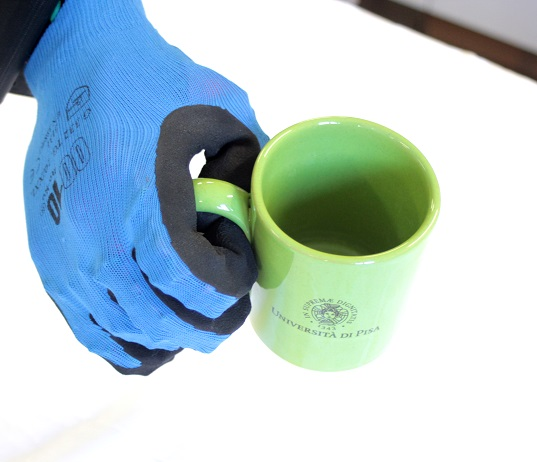
\includegraphics[width=0.45\linewidth]{mug_1_small.jpg} &
  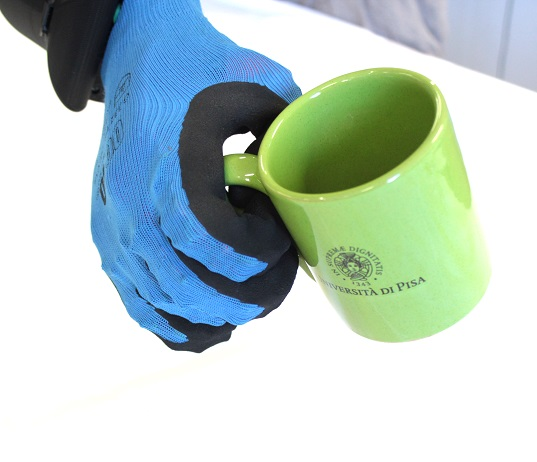
\includegraphics[width=0.45\linewidth]{mug_2_small.jpg} \\
  \end{tabular}
 \caption{{We want transferrable grasps that are robust to different initial hand-object poses, and thus different interactions during reach to grasp, thus reaching similar final grasp states. We achieve this by learning a set of trajectories that, associated with a model of the final grasp state, form an attractor basin around that state.}}
  \label{fig:two_grasps}
\end{figure}

One approach would be to learn the typical contact interactions that occur during a grasp, and to generate new grasps that reproduce these. The contact interactions are, however, rather complex and variable, even given small variations in object shape and friction. Therefore we tackle the problem by implicitly encoding the contact interactions in terms of the approach trajectory. Our method learns both the desired final contacts, the final hand shape, and possible sequences of hand pose during the reach to grasp trajectory. We build on our previous work on one-shot learning of grasps that transfer to novel objects, employing a product of experts. The novel technical contribution is that in this paper we show how to learn not only final grasp, but also the approach trajectory and control strategy for closing the dexterous hand. In particular, we learn a bundle of multiple trajectories that will all likely lead to a similar final stable grasp. We enable this by learning from examples generated in a rigid body physics simulation. Finally, at the grasp selection stage we now optimise across a space defined by this bundle of approach trajectories so as to maximise the chance of reaching a stable grasp. The method copes with partial and noisy shape information for the test objects. 

% SUBSECTION BETTER?

\subsection{Related Work}
Previous work in learning generalisable grasps falls broadly into two classes. One class of approaches utilises the shape of common object parts or their appearance to generalise grasps across object categories \cite{saxena2008b,detry2013a,herzog2014a, kroemer2012a}. This works well for low DoF hands. Another class of approaches captures the global properties of the hand shape either at the point of grasping, or during the approach \cite{ben2012generalization}. This global hand shape can additionally be associated with global object shape, allowing generalisation by warping grasps to match warps of global object shape \cite{hillenbrand2012transferring}. This second class works well for high DoF hands, but generalisation is more limited. We have previously achieved the advantages of both classes, generalising grasps across object categories with high DoF hands. In this paper we go beyond this, learning and generalising grasps for under-actuated hands.

Several hands with such behavior have been proposed in the literature with different implementations~\cite{Catalano2014Adaptive, Dollar2010Highly}, with a common goal: simplicity plus robustness. Their initial tests under human operation are promising, but autonomous grasping with underactuated hands faces challenges due to the almost non-observability of the finger deformation when the hand is constrained by the environment and/or a target object. Most of the existing planning algorithms for this type of hands boil down to generating good wrist poses and let the adaptive mechanism handle all variation and uncertainty while closing, such as~\cite{Eppner2015Planning}, where a sequence of wrist and object poses and the corresponding interaction wrenches are generated, which are expected to exploit environmental constraints. Another approach is that by~\cite{Bonilla2015Grasp}, where static wrist poses are sampled using different strategies around the object from where the fingers are closed using a rigid-body simulator, to finally select the areas of major success rate to generate new wrist poses.

While these approaches exploit, to some extent, the adaptive properties of the underactuated mechanism, they can be improved on. In this paper we show how we can, for the first time, learn grasps for underactuated hands that are then transferred to novel objects. This requires learning representations of the final grasp state that are amenable to transfer to new objects, grouping example grasps by the end grasp state, and learning and optimisation of reach-to-grasp trajectories.
